\documentclass[conference,a4paper]{IEEEtran}

\usepackage[utf8]{inputenc}
\usepackage{amsmath}
\usepackage{graphicx}
\usepackage[kw]{pseudo}
\usepackage{booktabs}
\usepackage{cite}
\usepackage{tikz}
\usetikzlibrary{arrows.meta,positioning}

\def\abstractname{Resumen}
\def\IEEEkeywordsname{Palabras clave}
\def\refname{Referencias}
\def\figurename{Fig.}
\def\tablename{TABLA}

\begin{document}

\title{Aprendizaje de una funcion de valor para jugar a Otelo con UCT}

\author{
  \IEEEauthorblockN{Fernando Pineda Muñoz}
  \IEEEauthorblockA{
    \textit{Ingeniería Informática - Ingeniería del Software}\\
    \textit{Universidad de Sevilla}\\
    Sevilla, España\\
    ferpinmun@alum.us.es\\
    fernaandopineda@gmail.com.es}
  
  \and
  
  \IEEEauthorblockN{Francisco Javier Hernandez-Vaquero Garrido}
  \IEEEauthorblockA{
    \textit{Ingeniería Informática - Ingeniería del Software}\\
    \textit{Universidad de Sevilla}\\
    Sevilla, España\\
    frahergar@alum.us.es\\
    javaquerog05@gmail.com.es}
}

\maketitle

\begin{abstract}
Este trabajo presenta el desarrollo de un agente inteligente para el juego de
Otelo mediante la combinacion de Monte Carlo Tree Search, la regla UCT y una red
neuronal de valor. El objetivo es obtener un jugador capaz de seleccionar
movimientos competitivos sin usar una heuristica manual como evaluador principal.

La implementacion incluye el motor completo del juego, varios agentes de
referencia, generacion de datos por autojuego, entrenamiento supervisado de una
red neuronal y una bateria de experimentos entre jugadores. En los experimentos
realizados, UCT con 16 iteraciones supera a un jugador voraz por 6 victorias a 2
y el agente UCT con red neuronal empata en victorias frente a UCT basico. Frente
al mismo rival voraz, el agente neuronal fue mucho mas rapido, aunque obtuvo
peor resultado deportivo con el dataset pequeno usado.
\end{abstract}

\begin{IEEEkeywords}
Otelo, Reversi, busqueda adversaria, Monte Carlo Tree Search, UCT, redes
neuronales, aprendizaje supervisado.
\end{IEEEkeywords}

\section{Introduccion}

Otelo, tambien conocido como Reversi, es un juego determinista, de suma cero y
con informacion perfecta. Estas propiedades lo convierten en un dominio adecuado
para estudiar tecnicas de busqueda adversaria y aprendizaje automatico. Aunque
el espacio de estados de Otelo es menor que el de Go, sigue siendo demasiado
grande para resolverlo exhaustivamente durante una partida real.

El objetivo del trabajo es implementar un agente basado en Monte Carlo Tree
Search (MCTS) con seleccion Upper Confidence bounds applied to Trees (UCT). La
version basica usa simulaciones aleatorias como politica por defecto, mientras
que la version avanzada reemplaza dicha politica por una red neuronal que estima
el valor de una posicion. Este planteamiento sigue de forma simplificada la idea
general de combinar busqueda y aprendizaje que aparece en AlphaGo y
AlphaZero~\cite{silver2016, silver2017}.

El interes del problema no esta solo en obtener un programa capaz de jugar, sino
en estudiar como se pueden combinar dos familias de tecnicas vistas en la
asignatura. Por un lado, la busqueda adversaria permite razonar explicitamente
sobre las consecuencias de las acciones disponibles. Por otro lado, el
aprendizaje automatico permite construir una funcion de evaluacion a partir de
datos, evitando disenar manualmente todos los criterios estrategicos del juego.
En este trabajo se ha mantenido una separacion clara entre ambos componentes:
el algoritmo UCT es responsable de explorar alternativas, mientras que la red
neuronal proporciona una estimacion rapida del valor de los estados.

La implementacion se ha desarrollado buscando tres objetivos practicos. El
primero es la correccion de las reglas, porque cualquier error en la generacion
de movimientos invalidaria tanto el entrenamiento como los torneos. El segundo
es la reproducibilidad: todos los experimentos se pueden lanzar mediante
comandos de consola con semillas fijas y los resultados quedan guardados en
ficheros estructurados. El tercero es la facilidad de defensa, de modo que cada
modulo del codigo tenga una responsabilidad concreta y pueda explicarse de forma
independiente.

El documento se organiza de la siguiente forma. En la seccion de preliminares se
describen las reglas de Otelo, MCTS, UCT y la red neuronal de valor. La seccion
de implementacion detalla la estructura del codigo y las decisiones de diseno.
La seccion de pruebas y experimentacion presenta el procedimiento seguido para
generar datos, entrenar el modelo y comparar agentes. Finalmente, se resumen las
conclusiones y las principales lineas de mejora.

\section{Preliminares}

\subsection{Reglas y representacion}

El tablero se representa como una matriz de tamano \(8 \times 8\). Internamente
se usa \(1\) para negras, \(-1\) para blancas y \(0\) para casillas vacias. Para
el dataset se puede exportar tambien la codificacion del enunciado:
\(0\) vacia, \(1\) blanca y \(2\) negra.

Un movimiento es legal si coloca una ficha en una casilla vacia y captura al
menos una ficha rival en direccion horizontal, vertical o diagonal. Si un
jugador no tiene movimientos legales debe pasar. La partida termina cuando el
tablero esta lleno o cuando ambos jugadores no tienen movimientos legales.

La implementacion comprueba las ocho direcciones posibles desde la casilla
candidata. En cada direccion se exige encontrar primero una o mas fichas rivales
y, a continuacion, una ficha propia que cierre la linea. Solo entonces las
fichas intermedias se consideran capturadas. Esta comprobacion se usa tanto para
determinar los movimientos legales como para aplicar una jugada, lo que reduce
la posibilidad de inconsistencias entre ambas operaciones.

Para entrenar la red no se usa directamente la matriz con valores \(1\), \(-1\)
y \(0\). En su lugar, cada posicion se transforma a una representacion desde la
perspectiva del jugador activo. Los primeros 64 atributos indican que casillas
contienen fichas propias y los 64 restantes indican que casillas contienen
fichas rivales. Esta codificacion evita que la red tenga que aprender dos casos
separados para blancas y negras, porque siempre interpreta la entrada desde el
punto de vista del jugador al que le toca mover.

\subsection{Monte Carlo Tree Search y UCT}

MCTS construye un arbol de busqueda de manera incremental. Cada iteracion
contiene cuatro fases: seleccion, expansion, simulacion y retropropagacion. En
la fase de seleccion se emplea UCT para equilibrar explotacion y exploracion:

\begin{equation}
UCT(s,a) = Q(s,a) + c \sqrt{\frac{\ln N(s)}{N(s,a)}}.
\end{equation}

En esta implementacion se usa una version negamax. Cada nodo almacena el valor
medio desde la perspectiva del jugador que debe mover en ese nodo. Por tanto,
cuando el padre selecciona un hijo, interpreta el valor del hijo con signo
opuesto.

La fase de seleccion recorre el arbol escogiendo en cada nodo el hijo con mayor
valor UCT. El primer termino, \(Q(s,a)\), representa el valor medio observado al
escoger la accion \(a\) desde el estado \(s\). El segundo termino aumenta el
atractivo de acciones poco visitadas y depende de \(N(s)\), el numero de visitas
del nodo padre, y \(N(s,a)\), el numero de visitas del hijo. La constante \(c\)
controla el equilibrio entre explotacion y exploracion; se ha usado el valor
\(\sqrt{2}\), habitual como punto de partida.

La politica por defecto de MCTS es especialmente importante. En la version
clasica, cuando se alcanza un nodo nuevo, se juega una partida simulada hasta el
final mediante decisiones aleatorias. El resultado de esa simulacion se
retropropaga por el arbol. En Otelo estas simulaciones son relativamente baratas,
pero siguen consumiendo tiempo y pueden producir estimaciones ruidosas. Por ello
la version con red neuronal sustituye la simulacion completa por una prediccion
del valor del estado.

\begin{figure}[t]
\centering
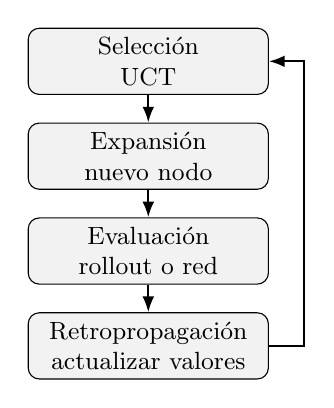
\begin{tikzpicture}[
  node distance=0.35cm,
  phase/.style={draw, rounded corners, align=center, minimum width=3.05cm,
    minimum height=0.58cm, fill=gray!10, font=\small},
  arrow/.style={-{Latex[length=2mm]}, thick}
]
\node[phase] (selection) {Selección\\UCT};
\node[phase, below=of selection] (expansion) {Expansión\\nuevo nodo};
\node[phase, below=of expansion] (evaluation) {Evaluación\\rollout o red};
\node[phase, below=of evaluation] (backprop) {Retropropagación\\actualizar valores};
\draw[arrow] (selection) -- (expansion);
\draw[arrow] (expansion) -- (evaluation);
\draw[arrow] (evaluation) -- (backprop);
\draw[arrow] (backprop.east) -- ++(0.45,0) |- (selection.east);
\end{tikzpicture}
\caption{Fases principales de una iteracion de MCTS con UCT.}
\label{fig:fases-uct}
\end{figure}

\subsection{Red neuronal de valor}

La red neuronal resuelve una tarea de regresion supervisada. La entrada contiene
128 atributos: un canal binario para las fichas propias y otro canal binario
para las fichas rivales. La salida es un numero real en \([-1, 1]\), obtenido con
una activacion \texttt{tanh}. El valor objetivo es \(+1\) si el jugador activo en
ese estado gano la partida, \(0\) si empato y \(-1\) si perdio.

Aunque el enunciado menciona herramientas como TensorFlow, la red se ha
implementado con NumPy para mantener el proyecto ligero y completamente
ejecutable en el entorno disponible. La arquitectura usada en el experimento
final tiene dos capas ocultas densas de 64 y 32 neuronas, activacion ReLU en las
capas ocultas y activacion \texttt{tanh} en la salida. El entrenamiento usa error
cuadratico medio y descenso de gradiente por mini-lotes mediante
retropropagacion.

\begin{table}[h]
\centering
\caption{Arquitectura de la red de valor.}
\label{tab:red}
\begin{tabular}{lll}
\toprule
Capa & Tamano & Activacion \\
\midrule
Entrada & 128 & -- \\
Oculta 1 & 64 & ReLU \\
Oculta 2 & 32 & ReLU \\
Salida & 1 & tanh \\
\bottomrule
\end{tabular}
\end{table}

\begin{figure}[t]
\centering
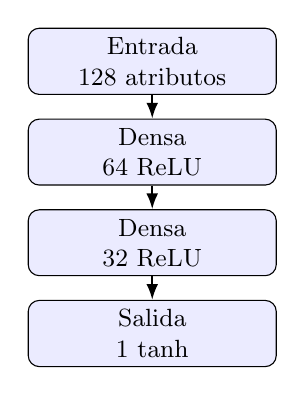
\begin{tikzpicture}[
  node distance=0.3cm,
  layer/.style={draw, rounded corners, align=center, minimum width=3.15cm,
    minimum height=0.58cm, fill=blue!8, font=\small},
  arrow/.style={-{Latex[length=2mm]}, thick}
]
\node[layer] (input) {Entrada\\128 atributos};
\node[layer, below=of input] (h1) {Densa\\64 ReLU};
\node[layer, below=of h1] (h2) {Densa\\32 ReLU};
\node[layer, below=of h2] (output) {Salida\\1 tanh};
\draw[arrow] (input) -- (h1);
\draw[arrow] (h1) -- (h2);
\draw[arrow] (h2) -- (output);
\end{tikzpicture}
\caption{Esquema de la red neuronal de valor utilizada.}
\label{fig:red-valor}
\end{figure}

El valor predicho no debe interpretarse como una probabilidad calibrada en
sentido estadistico estricto, sino como una estimacion normalizada de ventaja
para el jugador activo. Valores cercanos a \(1\) indican posiciones que la red
considera favorables, valores cercanos a \(-1\) posiciones desfavorables y
valores proximos a \(0\) posiciones equilibradas o inciertas.

\subsection{Trabajo relacionado}

La busqueda adversaria clasica, incluyendo minimax y poda alfa-beta, se estudia
habitualmente como punto de partida para juegos deterministas de dos jugadores
con informacion perfecta~\cite{russell2020}. Estos metodos exploran el arbol de
juego de manera sistematica, pero necesitan funciones heuristicas cuando no es
posible llegar hasta estados terminales. En Otelo, como en ajedrez o Go, la
profundidad completa de la partida hace inviable una expansion exhaustiva en
tiempo real.

MCTS ofrece una alternativa mas flexible porque concentra el esfuerzo en las
ramas que parecen mas prometedoras segun la experiencia acumulada durante las
simulaciones. El articulo de Browne et al.~\cite{browne2012} resume variantes
de MCTS y presenta UCT como una forma efectiva de resolver el dilema entre
explorar acciones poco probadas y explotar acciones con buenos resultados
previos. Esta idea encaja bien con juegos como Otelo, donde el factor de
ramificacion cambia mucho a lo largo de la partida.

Los trabajos de AlphaGo y AlphaZero muestran que las redes neuronales pueden
mejorar la busqueda cuando aprenden a evaluar posiciones o a priorizar
movimientos~\cite{silver2016, silver2017}. La propuesta desarrollada aqui no
pretende reproducir esos sistemas, que usan arquitecturas profundas, grandes
cantidades de computo y entrenamiento iterativo. La contribucion de este trabajo
es una version reducida y explicable: UCT proporciona la busqueda y una red de
valor sencilla sustituye la simulacion aleatoria de la politica por defecto.

\section{Implementacion}

El proyecto se organiza como un paquete Python. El modulo \texttt{game.py}
implementa las reglas, \texttt{mcts.py} implementa UCT, \texttt{agents.py}
define los jugadores, \texttt{self\_play.py} genera datasets,
\texttt{neural.py} entrena la red de valor y \texttt{tournament.py} ejecuta
comparativas.

\subsection{Motor del juego}

El motor del juego se implementa en la clase \texttt{OthelloState}. Cada estado
contiene el tablero, el jugador activo y el numero de pases consecutivos. Esta
ultima variable permite detectar correctamente el final de la partida cuando
ambos jugadores pasan. Los estados se tratan como objetos inmutables: al aplicar
una jugada se crea un nuevo estado con un tablero copiado. Esta decision aumenta
el coste de memoria, pero simplifica la busqueda porque los nodos del arbol no
comparten tableros modificables.

El modulo tambien incluye funciones auxiliares para convertir coordenadas de
texto, calcular puntuaciones, representar el tablero en ASCII y obtener
caracteristicas para la red. La interfaz de texto muestra con asteriscos las
jugadas legales, lo que permite probar el agente sin necesidad de construir una
interfaz grafica.

\subsection{Agentes implementados}

Se han implementado varios agentes para disponer de rivales de dificultad
creciente. El agente aleatorio elige uniformemente una accion legal y sirve como
baseline minimo. El agente voraz selecciona la jugada que voltea mas fichas en
el movimiento inmediato. El agente heuristico combina diferencia de fichas,
movilidad y esquinas. Finalmente, los agentes UCT y UCTNN usan busqueda de arbol
con la diferencia de que UCTNN recibe una red neuronal entrenada como evaluador.

Disponer de estos agentes facilita el analisis experimental. Si el agente UCT no
superase al aleatorio o al voraz, probablemente habria un error en la busqueda o
en las reglas. Si UCTNN no mejorase a los baselines, la causa podria estar en la
calidad del dataset, en la arquitectura de la red o en la integracion con MCTS.

El agente heuristico no forma parte del requisito principal de junio, pero se
incluyo para disponer de una referencia intermedia entre el agente voraz y UCT.
Su evaluacion combina tres criterios. La diferencia de fichas mide la ventaja
material actual; la movilidad mide cuantas acciones legales conserva cada
jugador; y las esquinas capturan un aspecto estrategico importante, ya que una
ficha situada en una esquina no puede ser volteada posteriormente. La ponderacion
usada no se ha optimizado automaticamente, sino que se ha elegido como una
heuristica simple y explicable.

Esta variedad de agentes tambien permite detectar comportamientos anomalos. Por
ejemplo, un agente que gana al aleatorio pero pierde claramente contra el voraz
puede estar tomando decisiones localmente razonables pero estrategicamente
debiles. Un agente que mejora al voraz pero no escala al aumentar iteraciones
puede estar limitado por la politica por defecto. Estas comparaciones son
importantes porque una unica partida aislada no permite evaluar de forma fiable
la calidad de un jugador.

\subsection{Integracion de la red en UCT}

La integracion se realiza mediante un parametro \texttt{evaluator} en la clase
\texttt{UCTSearch}. Si este parametro es nulo, la evaluacion de un nodo no
terminal se obtiene mediante la politica por defecto, que realiza una simulacion
hasta el final de la partida o hasta un limite de profundidad. Si el parametro
contiene una funcion, UCT llama directamente a esa funcion y limita el resultado
al intervalo \([-1,1]\). El agente UCTNN pasa como evaluador una llamada a
\texttt{network.predict\_state}.

Esta decision evita duplicar el codigo de MCTS: el mismo algoritmo sirve para la
version clasica y para la version neuronal. La diferencia de comportamiento
queda localizada en la funcion de evaluacion, que es precisamente el punto que
pide modificar el enunciado de la convocatoria de junio.

\begin{figure*}[t]
\begin{pseudo}*
\hd{\fn{UCT}}(estado, iters) \\*
\textbf{Entrada}: estado actual del juego \\
\textbf{Salida}: movimiento seleccionado \\
raiz \(\leftarrow\) nuevo nodo con estado \\
repetir \(iters\) veces \\+
  nodo \(\leftarrow\) \fn{seleccion}(raiz) \\
  si nodo no es terminal entonces \\+
    nodo \(\leftarrow\) \fn{expandir}(nodo) \\-
  valor \(\leftarrow\) \fn{eval}(nodo.estado) \\
  \fn{backprop}(nodo, valor) \\-
devolver mejor hijo de raiz
\end{pseudo}
\caption{Esquema del algoritmo UCT implementado.}
\label{pcd:uct}
\end{figure*}

La politica por defecto de la version basica realiza una simulacion aleatoria
hasta final de partida. La version con red neuronal sustituye esa simulacion por
una llamada al modelo de valor, reduciendo el coste de evaluacion y guiando la
busqueda hacia posiciones aprendidas mediante autojuego.

\subsection{Generacion de datos}

El dataset se genera mediante partidas automaticas entre dos copias del mismo
agente. Durante cada partida se guardan los estados intermedios despues de cada
movimiento. Al finalizar, cada estado recibe como etiqueta el resultado de la
partida desde la perspectiva del jugador activo en ese estado. De esta forma, el
mismo tablero puede tener interpretaciones distintas si cambia el jugador al que
le toca mover.

Para aumentar el numero de ejemplos se aplican las ocho simetrias del tablero:
cuatro rotaciones y sus reflejos horizontales. Estas transformaciones conservan
el resultado estrategico de la posicion, por lo que permiten aumentar el dataset
sin generar nuevas partidas. En el experimento final, 12 partidas de autojuego
produjeron 5720 ejemplos tras aplicar estas simetrias.

\begin{figure*}[t]
\centering
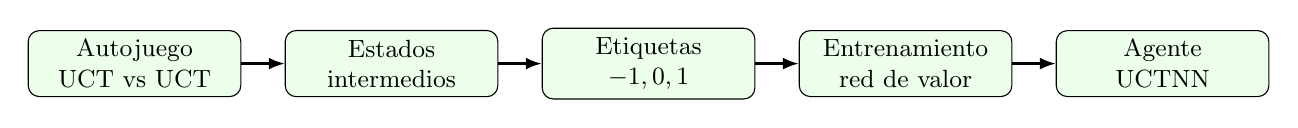
\begin{tikzpicture}[
  node distance=0.55cm,
  block/.style={draw, rounded corners, align=center, minimum width=2.7cm,
    minimum height=0.75cm, fill=green!8, font=\small},
  arrow/.style={-{Latex[length=2mm]}, thick}
]
\node[block] (selfplay) {Autojuego\\UCT vs UCT};
\node[block, right=of selfplay] (states) {Estados\\intermedios};
\node[block, right=of states] (labels) {Etiquetas\\$-1,0,1$};
\node[block, right=of labels] (training) {Entrenamiento\\red de valor};
\node[block, right=of training] (agent) {Agente\\UCTNN};
\draw[arrow] (selfplay) -- (states);
\draw[arrow] (states) -- (labels);
\draw[arrow] (labels) -- (training);
\draw[arrow] (training) -- (agent);
\end{tikzpicture}
\caption{Flujo completo de generacion de datos, entrenamiento y uso del modelo.}
\label{fig:flujo-experimental}
\end{figure*}

\subsection{Reproducibilidad}

Los experimentos se agrupan en el modulo \texttt{experiments.py}. Este script
genera el dataset, entrena la red, ejecuta los torneos y escribe los resultados
en formato Markdown y JSON. Ademas, todas las llamadas usan semillas
configurables. Esto permite repetir la misma ejecucion durante la defensa o
modificar facilmente el numero de partidas, epocas o iteraciones UCT.

\begin{table}[h]
\centering
\caption{Artefactos principales generados por el proyecto.}
\label{tab:artefactos}
\begin{tabular}{ll}
\toprule
Fichero & Contenido \\
\midrule
\texttt{selfplay\_experiment.npz} & Dataset de estados y etiquetas \\
\texttt{value\_net\_experiment.npz} & Pesos de la red entrenada \\
\texttt{experiment\_results.md} & Resumen legible de torneos \\
\texttt{experiment\_results.json} & Resultados estructurados \\
\texttt{memoria-otelo.pdf} & Documento final compilado \\
\bottomrule
\end{tabular}
\end{table}

Los ficheros \texttt{npz} se han elegido porque permiten almacenar varios
arrays NumPy comprimidos en un unico archivo. El dataset contiene los atributos
\texttt{x}, las etiquetas \texttt{y} y metadatos sobre el agente usado para el
autojuego. El modelo contiene el tamano de entrada, las capas ocultas y las
matrices de pesos y sesgos de cada capa. Esta separacion permite regenerar el
modelo desde cero o reutilizar uno ya entrenado en torneos posteriores.

\subsection{Coste computacional}

El coste de una decision UCT depende principalmente del numero de iteraciones y
del coste de evaluar cada nodo expandido. En la version basica, cada evaluacion
puede implicar una simulacion completa de partida. Aunque Otelo tiene un tablero
pequeno, una simulacion puede contener decenas de movimientos y cada movimiento
requiere volver a calcular acciones legales. Por ello, aumentar el numero de
iteraciones mejora la calidad de la busqueda, pero tambien incrementa
rapidamente el tiempo por jugada.

La version neuronal modifica este equilibrio. Evaluar una posicion con la red
consiste en varias multiplicaciones matriciales pequenas: \(128 \times 64\),
\(64 \times 32\) y \(32 \times 1\). Este coste es mucho mas estable que una
simulacion aleatoria completa. La desventaja es que la evaluacion deja de ser
una muestra directa del resultado de una partida y pasa a depender de la calidad
del entrenamiento. En otras palabras, UCT basico suele ser mas caro pero menos
sesgado por el dataset; UCTNN es mas rapido, pero puede equivocarse
sistematicamente si la red ha aprendido mal ciertas posiciones.

\begin{table}[h]
\centering
\caption{Comparacion cualitativa de evaluadores dentro de UCT.}
\label{tab:evaluadores}
\begin{tabular}{lll}
\toprule
Evaluador & Ventaja & Riesgo \\
\midrule
Rollout & No requiere datos & Coste alto y ruido \\
Heuristica & Muy rapido & Diseno manual \\
Red valor & Rapido y aprendido & Depende del dataset \\
\bottomrule
\end{tabular}
\end{table}

En los resultados obtenidos se aprecia esta diferencia. El torneo UCT-16 contra
Greedy tardo 24.4 segundos, mientras que UCTNN-16 contra Greedy tardo 1.7
segundos. La comparacion no mide solo una jugada, pero si muestra que sustituir
rollouts por una red reduce mucho el tiempo total de juego. La cuestion abierta
es mejorar la calidad del evaluador neuronal para que esa ganancia de velocidad
no implique perder fuerza de juego.

\section{Pruebas y experimentacion}

Se han preparado pruebas unitarias para verificar los movimientos legales
iniciales, el volteo de fichas, la obligacion de pasar, la deteccion de final de
partida y la integracion basica de UCT. Estas pruebas se ejecutan con:

\begin{verbatim}
python3 -m unittest discover -s tests -v
\end{verbatim}

En la ejecucion realizada se superaron 8 pruebas unitarias. Estas pruebas no
demuestran que el agente sea optimo, pero si reducen el riesgo de fallos
basicos en el motor: movimientos iniciales incorrectos, volteos mal aplicados,
pases ilegales o partidas que no terminan. Tambien se verifica que UCT siempre
devuelve una accion legal en el estado inicial y que la red puede realizar al
menos una iteracion de entrenamiento.

\subsection{Diseno experimental}

Los torneos alternan el color inicial entre agentes para reducir el sesgo de que
negras muevan primero. La medida principal es el numero de victorias, derrotas y
empates. Como medida secundaria se usa la diferencia media de fichas desde la
perspectiva del agente A, porque permite distinguir victorias ajustadas de
victorias amplias. Tambien se registra el tiempo total de cada torneo para
comparar el coste de los distintos evaluadores.

El experimento reproducible se ejecuto con el siguiente comando:

\begin{verbatim}
python3 -m othello_ai.experiments \
  --selfplay-games 12 \
  --selfplay-agent uct:12 \
  --epochs 20 \
  --tournament-games 8 \
  --uct-iters 16 \
  --seed 23
\end{verbatim}

La configuracion se eligio como compromiso entre tiempo de ejecucion y
capacidad de obtener resultados interpretables en un entorno local. El numero de
partidas de entrenamiento es pequeno, por lo que los resultados no deben
entenderse como una medida definitiva de fuerza de juego, sino como una prueba
completa del pipeline solicitado: autojuego, aprendizaje, integracion con UCT y
comparacion entre agentes.

\begin{table}[h]
\centering
\caption{Configuracion y resultado del entrenamiento.}
\label{tab:entrenamiento}
\begin{tabular}{lr}
\toprule
Magnitud & Valor \\
\midrule
Partidas de autojuego & 12 \\
Agente de autojuego & UCT-12 \\
Ejemplos generados & 5720 \\
Capas ocultas & 64, 32 \\
Epocas & 20 \\
Loss entrenamiento & 0.84350 \\
Loss validacion & 0.87669 \\
\bottomrule
\end{tabular}
\end{table}

El conjunto de entrenamiento se genero por autojuego usando UCT con 12
iteraciones por decision. Cada estado intermedio se etiqueto con el resultado
final desde la perspectiva del jugador activo y se aplicaron las ocho simetrias
del tablero. La perdida de validacion bajo de 1.03280 a 0.87669, lo que indica
que la red aprende una senal util, aunque todavia limitada por el tamano pequeno
del dataset.

\begin{table*}[t]
\centering
\caption{Resultados de los torneos. La diferencia media se mide desde la perspectiva del agente A.}
\label{tab:torneos}
\begin{tabular}{llrrrrr}
\toprule
Agente A & Agente B & Partidas & Victorias A & Victorias B & Empates & Dif. media A \\
\midrule
Greedy & Random & 8 & 5 & 3 & 0 & 7.50 \\
Heuristico & Greedy & 8 & 7 & 1 & 0 & 18.00 \\
UCT-16 & Greedy & 8 & 6 & 2 & 0 & 9.00 \\
UCT-32 & UCT-16 & 8 & 4 & 3 & 1 & 6.00 \\
UCTNN-16 & Random & 8 & 7 & 1 & 0 & 13.00 \\
UCTNN-16 & Greedy & 8 & 3 & 4 & 1 & -6.75 \\
UCTNN-16 & UCT-16 & 8 & 4 & 4 & 0 & -0.25 \\
\bottomrule
\end{tabular}
\end{table*}

La tabla~\ref{tab:torneos} muestra tres conclusiones principales. En primer
lugar, las heuristicas simples ya son claramente superiores al jugador aleatorio,
por lo que son buenos rivales de control. En segundo lugar, UCT mejora al jugador
voraz incluso con solo 16 iteraciones, y aumentar a 32 iteraciones produce una
ligera mejora frente a UCT-16. En tercer lugar, UCTNN-16 es competitivo con
UCT-16 en numero de victorias, pero no supera aun al jugador voraz. Este ultimo
resultado es razonable: la red se entreno con solo 12 partidas de autojuego, por
lo que todavia no dispone de suficientes ejemplos para generalizar bien todas las
fases de la partida.

Tambien se observa una diferencia clara de coste temporal. El torneo UCT-16
contra Greedy tardo 24.4 segundos, mientras que el torneo UCTNN-16 contra Greedy
tardo 1.7 segundos. Esta diferencia aparece porque la red sustituye las
simulaciones aleatorias completas de la politica por defecto por una evaluacion
directa del estado.

\subsection{Analisis de errores y limitaciones}

El resultado mas importante desde el punto de vista critico es que UCTNN-16 no
supera al agente voraz en el experimento realizado. Esto no contradice el
planteamiento del trabajo, sino que muestra una limitacion razonable de la
configuracion usada. La red se entrena con pocos ejemplos y estos ejemplos
proceden de un agente UCT debil, con solo 12 iteraciones por decision durante el
autojuego. Por tanto, el modelo aprende una senal aproximada, pero no una
estrategia suficientemente robusta para todas las fases de la partida.

Otra limitacion es que la red predice solo el valor del estado, no una politica
de movimientos. Esto significa que UCTNN sigue expandiendo acciones sin una guia
neuronal directa sobre que jugadas son mas prometedoras. En sistemas como
AlphaZero se aprenden simultaneamente una politica y una funcion de valor, lo
que permite dirigir mucho mejor la busqueda. En este trabajo se ha mantenido una
version mas sencilla porque el objetivo de la convocatoria es reemplazar la
politica por defecto de UCT por una red de evaluacion.

Por ultimo, el numero de partidas de torneo es bajo. Ocho partidas por
emparejamiento permiten observar tendencias, pero no proporcionan una estimacion
estadistica estable. Para una evaluacion mas fuerte seria conveniente repetir
los torneos con al menos 50 o 100 partidas por enfrentamiento y varias semillas
distintas.

\subsection{Amenazas a la validez}

La primera amenaza a la validez interna es la aleatoriedad. MCTS, los agentes
aleatorios y la inicializacion de la red dependen de semillas. Aunque los
experimentos fijan una semilla para poder reproducir los resultados, otras
semillas podrian producir variaciones, especialmente con tan pocas partidas. Por
ese motivo, las conclusiones se formulan como tendencias observadas y no como
afirmaciones absolutas sobre la fuerza de cada agente.

La segunda amenaza es el sesgo del generador de datos. Como el autojuego se
realizo con un agente UCT pequeno, las posiciones del dataset reflejan el estilo
de juego y los errores de ese agente. Si se generasen partidas con mas
iteraciones, con varios tipos de rivales o mediante reentrenamiento iterativo,
la red probablemente recibiria ejemplos mas variados y podria mejorar su
capacidad de generalizacion.

La tercera amenaza es la escala del entrenamiento. La red usada es pequena y el
dataset tambien. Esta decision fue adecuada para mantener el proyecto ejecutable
en un ordenador personal, pero limita la calidad del evaluador neuronal. Aun
asi, el experimento es suficiente para comprobar el requisito principal de la
convocatoria: disenar una red, entrenarla con estados de Otelo y usarla dentro
de MCTS como reemplazo de la politica por defecto.

\subsection{Uso durante la defensa}

El proyecto esta preparado para poder mostrar tres tipos de ejecucion durante la
defensa. La primera es una partida interactiva contra la maquina usando la
interfaz de texto. Esta ejecucion permite comprobar que el motor aplica las
reglas correctamente y que el agente devuelve movimientos legales. La segunda es
un torneo corto entre dos agentes, util para mostrar como se comparan los
jugadores sin intervencion humana. La tercera es la ejecucion del script de
experimentos, que reproduce el pipeline completo de generacion de datos,
entrenamiento y evaluacion.

Estas ejecuciones tambien ayudan a responder preguntas tecnicas. Si se pregunta
donde se sustituye la politica por defecto, la respuesta esta en el parametro
\texttt{evaluator} de UCT. Si se pregunta que contiene el modelo, se puede
mostrar que el archivo guarda unicamente matrices de pesos y vectores de sesgos.
Si se pregunta como se etiqueta un estado, se puede explicar que la etiqueta se
asigna al finalizar la partida, segun el resultado desde la perspectiva del
jugador activo en ese estado.

Una modificacion sencilla que podria pedirse en directo es cambiar el numero de
iteraciones de UCT o enfrentar otros agentes. El diseno por argumentos de linea
de comandos permite hacerlo sin tocar el codigo. Otra modificacion posible es
entrenar una red con mas epocas o con otro tamano de capas ocultas. Estos
parametros tambien estan expuestos en los scripts, de modo que el trabajo no
depende de valores fijados de forma rigida en el codigo.

\section{Conclusiones}

El proyecto implementa el pipeline completo solicitado para la convocatoria de
junio: reglas de Otelo, UCT, generacion de estados por autojuego, entrenamiento
de una red neuronal y uso de esa red como evaluador dentro de la busqueda. La
principal ventaja del enfoque es que separa claramente el motor del juego, la
busqueda y el aprendizaje, lo que facilita la defensa y la realizacion de
experimentos.

Los resultados muestran que UCT es una mejora solida sobre los baselines simples
y que la red neuronal aprende una funcion de valor con informacion util. Sin
embargo, el agente UCTNN entrenado con el dataset pequeno usado en esta prueba
solo iguala a UCT-16 y no supera al agente voraz. La interpretacion mas plausible
es que la calidad del evaluador neuronal depende fuertemente de la cantidad y
calidad del autojuego usado para entrenar.

Como trabajo futuro se propone aumentar el numero de partidas de entrenamiento,
comparar distintas arquitecturas de red, ajustar la constante de exploracion de
UCT y realizar reentrenamiento iterativo. Tambien seria posible aprender una
politica de movimientos ademas de la funcion de valor, acercando el sistema a
los enfoques usados en AlphaZero.

\section*{Uso de IA generativa}

Se utilizo Codex, basado en GPT-5, para leer el enunciado, proponer la
arquitectura, generar una primera version del codigo, preparar pruebas y crear
esta documentacion inicial. Los prompts principales fueron: ``Lee el pdf y dime
como crees que se podria hacer el mejor proyecto posible'' y ``Ejecutalo''. El
codigo y los resultados deben ser revisados y entendidos por todos los
integrantes antes de la defensa.

\begin{thebibliography}{00}
\bibitem{russell2020} S. Russell and P. Norvig, \emph{Artificial Intelligence:
A Modern Approach}, 4th ed. Pearson, 2020.
\bibitem{browne2012} C. B. Browne et al., ``A survey of Monte Carlo Tree Search
methods,'' \emph{IEEE Transactions on Computational Intelligence and AI in
Games}, vol. 4, no. 1, pp. 1--43, 2012.
\bibitem{silver2016} D. Silver et al., ``Mastering the game of Go with deep
neural networks and tree search,'' \emph{Nature}, vol. 529, pp. 484--489, 2016.
\bibitem{silver2017} D. Silver et al., ``Mastering Chess and Shogi by self-play
with a general reinforcement learning algorithm,'' arXiv:1712.01815, 2017.
\end{thebibliography}

\end{document}
